%============================================================================
% LaTeX File
% Daniel J. Greenhoe
%============================================================================
%======================================
\chapter{Random Sequences}
\label{app:random_processes}
%======================================
\qboxnpq
  {
    Ronald A. Fisher, 
    \href{http://www-history.mcs.st-andrews.ac.uk/Timelines/TimelineG.html}{(1890--1962)}, 
    Statistician,
    at a lecture in 1958 at Michigan State University
    \footnotemark
  }
  {../common/graphics/portraits/fisher_geneticsorg.jpg}
  {We are quite in danger of sending highly trained and highly intelligent 
  young men out into the world with tables of erroneous numbers under their arms, 
  and with a dense fog in the place where their brains ought to be. 
  In this century, of course, they will be working on guided missiles and advising the 
  medical profession on the control of disease, 
  and there is no limit to the extent to which they could impede every sort of national effort.}
  \footnotetext{
    quote:       \citePp{yates1963}{107}.
    image:       \url{http://www.genetics.org/content/154/4/1419}
    }

%=======================================
\section{Definitions}
%=======================================
%---------------------------------------
\begin{definition}
\label{def:randseq}
%---------------------------------------
\defboxt{
    A \fnctd{random sequence} $\rvx(n)\in\psO$ is a \fncte{sequence} \ifsxref{seq}{def:seq} 
  \\over a \structe{probability space} $\ps$ \xref{def:ps}.
  }
\end{definition}

%---------------------------------------
\begin{definition}
\footnote{
  \citerpgc{papoulis1984}{263}{0070484686}{$R_{xy}(m)=E\brb{\rvx(m)\rvy^\ast(0)}$},
  \citerpc{wilks1963}{77}{\textsection 3.4 ``Moments of two-dimensional random variables"},
  \citerpgc{cadzow}      {341}{0023180102}{$r_{xy}(m)=E\brs{\rvx(m)\rvy^\ast(0)}$},
  \citePc  {matlab_xcorr}                 {$R_{xy}(m)=E\setn{x_{n+m}y_n^\ast}   $},
  \citePc  {matlab_cpsd}                  {$R_{xy}(m)=E\setn{x_{n+m}y_n^\ast}   $}
  }
\label{def:pmeanxn}
\label{def:pvarxn}
\label{def:Rxxnm}
\label{def:Rxxnm}
\label{def:Ryynm}
\label{def:Rxynm}
%---------------------------------------
Let $\rvx(n)$ and $\rvy(n)$ be \fncte{random sequence}s.\\
\defbox{\begin{array}{MlMlc>{\ds}l}
     The \fnctd{mean}             & \pmeanx(n) & of $\rvx(n)$               is & \pmeanx(n)&\eqd& \pE\brs{\rvx(n)}
   \\The \fnctd{variance}         & \pvarx(n)  & of $\rvx(n)$               is & \pvarx(n) &\eqd& \pE\brp{\brs{\rvx(n)-\pmeanx(n)}^2}
   \\The \fnctd{cross-correlation}& \Rxy(n,m)  & of $\rvx(n)$ and $\rvy(n)$ is & \Rxy(n,m) &\eqd& \pE\brs{\rvx(n+m)\rvy^\ast(n)}
   \\The \fnctd{auto-correlation} & \Rxx(n,m)  & of $\rvx(n)$               is & \Rxx(n,m) &\eqd& \brlr{\Rxy(n,m)}_{\rvy=\rvx}
  %\\The \fnctd{auto-correlation operator} & \opR\ff    & of $\ff(t)$               is & \opR f    &\eqd& \int_{u\in\R}\Rxx(t,u) f(u) \du     %& \text{(\prope{auto-correlation operator})}
\end{array}}
\end{definition}

%---------------------------------------
\section{Properties}
%---------------------------------------
%---------------------------------------
\begin{theorem}
\label{thm:Rxxnm}
\label{thm:Ryynm}
\label{thm:Rxynm}
%---------------------------------------
\thmbox{\begin{array}{rcl}
   \Rxx(n,m) &=& \Rxx^\ast(n+m,-m)\\
   \Rxy(n,m) &=& \Ryx^\ast(n+m,-m)
\end{array}}
\end{theorem}
\begin{proof}
\begin{align*}
  \Rxy(n,m)
     &\eqd \pE\brs{\rvx(n+m) \rvy^\ast(n)}
     && \text{by definition of $\Rxy(n,m)$}
     && \text{\xref{def:Rxynm}}
   \\&= \pE\brs{\rvy^\ast(n) \rvx(n+m)}
     && \text{by \prope{commutative} property of $\fieldC$}
     && \text{\ifxref{algebra}{def:field}}
   \\&= \brp{\pE\brs{\rvy(n) \rvx^\ast(n+m)}}^\ast
     && \text{by \prope{distributive} property of \structd{$\invo$-algebra}s}
     && \text{\xref{def:staralg}}
   \\&= \brp{\pE\brs{\rvy(n+m-m) \rvx^\ast(n+m)}}^\ast
     && \text{by \prope{additive identity} property of $\fieldR$}
     && \text{\ifxref{algebra}{def:field}}
   \\&\eqd \Ryx^\ast(n+m,-m)
     && \text{by definition of $\Rxy(n,m)$}
     && \text{\xref{def:Rxynm}}
   \\
   \\
   \Rxx(n,m)
     &= \brlr{\Rxy(n,m)}_{\rvy=\rvx}
     && \text{by $\rvy=\rvx$ constraint}
   \\&= \brlr{\Rxy^\ast(n+m,-m)}_{\rvy=\rvx}
     && \text{by previous result}
   \\&= \Rxx^\ast(n+m,-m)
     && \text{by $\rvy=\rvx$ constraint}
\end{align*}
\end{proof}

%---------------------------------------
\section{Wide Sense Stationary processes}
\index{wide sense stationary}
\index{WSS}
%---------------------------------------
%---------------------------------------
\begin{definition}
%---------------------------------------
Let $\rvx(n)$ be a \fncte{random sequence} with \fncte{mean} $\pmeanx(n)$ and
\fncte{variance} $\pvar(n)$ \xref{def:pvarxn}.
\\
\defboxt{
  $\rvx(n)$ is \propd{wide sense stationary} (\propd{WSS}) if
  \\\indentx
    $\begin{array}{FlMMD}
       1. & \pmeanx(n)  & is \prope{constant} with respect to $n$ & (\prope{stationary in the 1st moment})    & and\\
       2. & \pvarx(n)   & is \prope{constant} with respect to $n$ & (\prope{stationary in the 2nd moment})
    \end{array}$
  }
\end{definition}

%---------------------------------------
\begin{definition}
\footnote{
  \citerpgc{papoulis1984}{263}{0070484686}{``$R_{xy}(\tau)=E\brb{\rvx(t+\tau)\rvy^\ast(t)}$"},
  %\citerpgc{kay1988}{52}{8131733564}{``$r_{xy}[k] = \mathcal{E}\brb{x^\ast[n]y[n+k]}\quad(3.42)"$},
  %\citerpgc{bendat2010}{111}{1118210824}{$R_{xy}(\tau)=E\brs{\rvx(t)\rvy(t+\tau)}$},
  \citerpgc{cadzow}{341}{0023180102}{$r_{xy}(n)=E\brs{\rvx(k+n)\rvy^\ast(k)}$ (10.41)}
  %\citerpgc{koopmans1995}{}{{0124192513}{}
  %\citerpgc{weisstein2002}{594}{1420035223}{entry: Cross-Correlation; $f\star g=\int_{-\infty}^{\infty}\bar{f}(\tau)g(t+\tau)\dtau$ (4)},
  %\citerpgc{bracewell1965}{46,243}{???}{cited by other reference} % https://books.google.com/books?id=oVFTDwAAQBAJ&pg=PA92&dq=bracewell+%22pentagram+notation%22&hl=en&sa=X&ved=0ahUKEwigptTEq-DeAhXIi60KHd1RCJIQ6AEILjAB#v=onepage&q=bracewell%20%22pentagram%20notation%22&f=false
  }
\label{def:mean_wss}
\label{def:Rxxm}
\label{def:Rxym}
%---------------------------------------
Let $\rvx(n)$ be a \fncte{random sequence} with statistics
$\pmeanx(n)$, $\pvarx(n)$, $\Rxx(n,m)$, and $\Rxy(n,m)$ \xref{def:Rxynm}.
\defboxt{
  $\brb{\begin{array}{M}
    $\rvx$ and $\rvy$ are
    \prope{wide sense stationary}
  \end{array}}\quad\implies$
  \\\quad$
  \brb{\begin{array}{FMlMlc>{\ds}l}
     (1).&The \fnctd{mean}              & \pmeanx  & of $\rvx(n)$               is & \pmeanx &\eqd& \pE\brs{\rvx(0)}
   \\(2).&The \fnctd{variance}          & \pvarx   & of $\rvx(n)$               is & \pvarx  &\eqd& \pE\brp{\brs{\rvx(0)-\pmeanx}^2}
   \\(4).&The \fnctd{cross-correlation} & \Rxy(m)  & of $\rvx(n)$ and $\rvy(n)$ is & \Rxy(m) &\eqd& \pE\brs{\rvx(m)\rvy^\ast(0)}
   \\(3).&The \fnctd{auto-correlation}  & \Rxx(m)  & of $\rvx(n)$               is & \Rxx(m) &\eqd& \brlr{\Rxy(m)}_{\rvy=\rvx}
  %\\The \fnctd{auto-correlation operator} & \opR\ff    & of $\ff(t)$               is & \opR f    &\eqd& \int_{u\in\R}\Rxx(t,u) f(u) \du     %& \text{(\prope{auto-correlation operator})}
\end{array}}$
  }
\end{definition}

%---------------------------------------
\begin{remark}
%---------------------------------------
  The $\Rxy(n,m)$ of \prefpp{def:Rxynm} and the $\Rxy(m)$ of \prefpp{def:Rxym} (etc.) are examples
  of \hie{function overload}---that is, functions that use the same
  mnemonic but are distinguished by different domains.
  Perhaps a more common example of function overload is the ``$+$" mnemonic.
  Traditionally it is used with domain of the natural numbers $\N$ as in $3+2$.
  Later it was extended for domain real numbers $\R$ as in $\sqrt{3}+\sqrt{2}$,
  or even complex numbers $\C$ as in $\brp{\sqrt{3}+i\sqrt{2}}+\brp{e+i\pi}$.
  And it was even more dramatically extended for use with domain $\R^\xN\times\R^\xM$
  in ``linear algebra" as in
  \\\indentx$
    \brs{\begin{array}{cc}1&2\\3&4\end{array}} +
    \brs{\begin{array}{cc}5&6\\7&8\end{array}} =
    \brs{\begin{array}{cc}6&8\\10&12\end{array}}
   $
\end{remark}

%---------------------------------------
\begin{remark}
\footnote{
  \citerppgc{marple1987}{51}{53}{9780132141499}{{\scshape``Appendix 2.A Source of Complex-Valued Signals"}},
  \citerppgc{marple2019}{48}{50}{9780486780528}{\textsection ``2.12 Extra: Source of Complex-Valued Signals"},
  \citerc{greenhoe_abcdc}{Chapter 2: Narrowband Signals}
  }
%---------------------------------------
The definition for $\Rxy(m)$ can be defined with the conjugate $\ast$ 
on either $\rvx$ or $\rvy$, or on neither or both; and moreover $\rvx$ may either lead or lag $\rvy$.
In total, there are $2\times2\times2=8$ different ways to define $\Rxy(m)$.\footnote{\citeP{greenhoe2019}}
and $\Rxx(m)$ involve complex numbers. 
This may seem curious when typical ADCs provide real-valued sequences.
Note however that complex-valued sequences often come up in signal processing due to 
some common system architectures:
\begin{enume}
  \item The presence of an \ope{FFT} operator in the signal processing path
  \item The \fncte{complex envelope} $\fx_l(t)$ of a modulated \prope{narrowband} communications signal $\fx(t)$.
  \item Communications channel processing involving phase discrimination (e.g. PSK and QAM).
\end{enume}

In the case of a narrowband signal $\fx(t)$ modulated by a sinusoid at center frequence $f_c$, 
we have three canonical forms. These can be shown to be equivalent:
\begin{align*}
  \fx(t)
    &\eqd \mcom{\boxed{\fa(t)\cos\brs{2\pi f_c t + \phi(t)}}}{amplitude-phase form}
    && \text{amplitude and phase form}
    %&& \text{\xref{def:cenv}}
  \\&= \mcom{\fa(t)\cos[\phi(t)]}{$\fp(t)$} \cos[2\pi f_c t]
      -\mcom{\fa(t)\sin[\phi(t)]}{$\fq(t)$} \sin[2\pi f_c t]
    && \text{by \thme{double angle formulas}}
    && \text{\ifxref{harTrig}{thm:trig_double}}
  \\&= \mcom{\boxed{\fp(t)\cos[2\pi f_c t] -\fq(t)\sin[2\pi f_c t]}}{quadrature form}
    && \text{quadrature form}
    %&& \text{\xref{def:cenv}}
  \\&= \Real\brp{[\fp(t)+i\fq(t)][\cos(2\pi f_c t) + i\sin(2\pi f_c t)]}
    && \text{by definitions of $\Real$}
    %&& \text{\xref{def:Re}}
  \\&= \mcom{\boxed{\Reb{\fx_l(t)e^{i2\pi f_c t}}}}{complex envelope form}
    && \text{by \thme{Euler's identity}}
    && \text{\ifxref{harTrig}{thm:eid}}
    %&& \text{complex envelope form}
    %&& \text{\xref{def:cenv}}
\end{align*}
Note that in these equivalent forms, the \fncte{complex envelope} $\fx_l(t)$ is conveniently represented
as a \prope{complex-valued} function in terms of the \fncte{quadrature component} $\fp(t)$ and the 
\fncte{inphase component} $\fq(t)$ such that $\fx_l(t)=\fp(t)+i\fq(t)$.
\end{remark}

%---------------------------------------
\begin{minipage}{\tw-60mm}
\begin{example}
%---------------------------------------
In practice (with real hardware), you will likely first have access to
the quadrature components $\fp(t)$ and $\fq(t)$.
Take for example the \hie{Analog Devices ADL5387 Quadrature Demodulator} and
evaluation board, as illustrated to the right.\footnotemark
Note that \fncte{quadrature component} $\fp(t)$ is available at connector ``Q OUTPUT"
     and  \fncte{inphase component}    $\fq(t)$ is available at connector ``I OUTPUT".
\end{example}
\end{minipage}\hfill\tbox{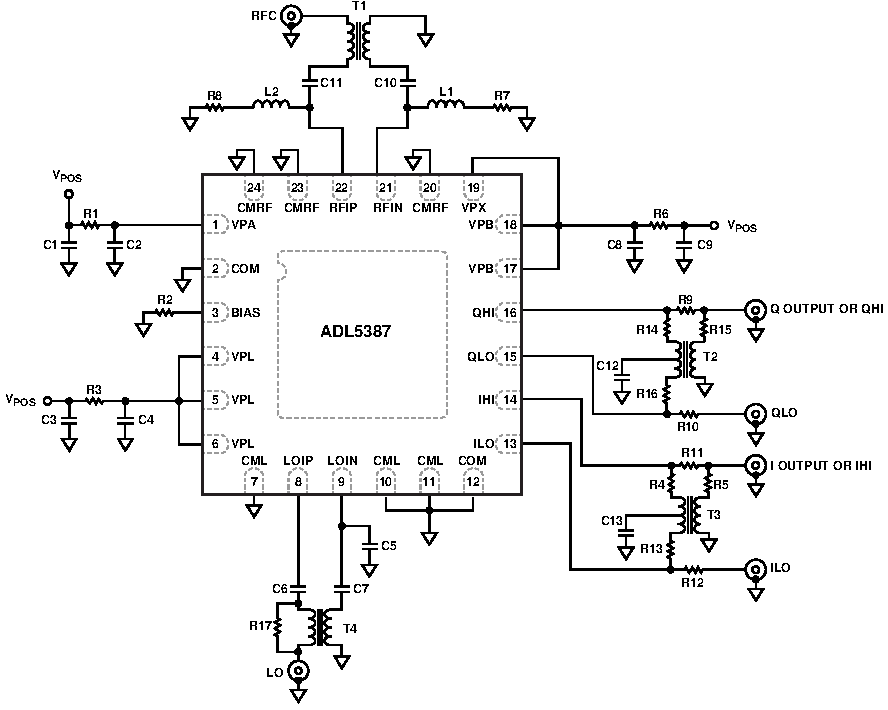
\includegraphics[width=55mm]{../common/ic/ADL5387_page24_schematic.pdf}}
\footnotetext{Diagram extracted from \citeP{ADL5387}.
Extraction notes: {\scriptsize
\verb|pdftk ADL5387.pdf cat 24 output page24.pdf|\\
\verb|pdfcrop --margins "-50 -120 -60 -260" --clip page24.pdf image.pdf|\\
\verb|gswin32c.exe -sDEVICE=pdfwrite -dNOPAUSE -dBATCH -dSAFER -dCompatibilityLevel=1.5 -sOutputFile=ADL5387_page24_schematic.pdf image.pdf| % https://superuser.com/questions/184288/how-to-convert-a-pdf-document-to-an-older-version
}}

%---------------------------------------
\begin{proposition}
\label{prop:Rxynmm}
\label{prop:Rxxnmm}
%---------------------------------------
Let $\rvy(n)$ be a \fncte{random sequence},
    $\rvx(n)$    a \fncte{random sequence} with \fncte{auto-correlation} $\Rxx(n,m)$,
and $\Rxy$    the \fncte{cross-correlation} of $\rvx$ and $\rvy$.
\propbox{
  \brb{\begin{array}{M}
    $\rvx$ and $\rvy$ are
    \\\prope{wide sense stationary}
    \\(\prope{WSS}) \xref{def:wss}
  \end{array}}
  \implies
  \brb{\begin{array}{rcll}
    \Rxx(n,m) &=& \Rxx(m) & \forall n\in\Z\\
    \Rxy(n,m) &=& \Rxy(m) & \forall n\in\Z\\
    \text{\xref{def:Rxynm}} && \text{\xref{def:Rxym}}
  \end{array}}
}
\end{proposition}
\begin{proof}
\begin{align*}
  \Rxy(n,m)
     &\eqd \pE\brs{\rvx[n+m]\rvy^\ast[n]}
     &&    \text{by definition of $\Rxy(n,m)$}
     &&    \text{\xref{def:Rxynm}}
   \\&=    \pE\brs{\rvx[n-n+m]\rvy^\ast[n-n]}
     &&    \text{by \prope{wide sense stationary} hypothesis}
   \\&=    \pE\brs{\rvx[m]\rvy^\ast[0]}
   \\&\eqd \Rxy(m)
     && \text{by definition of $\Rxy(m)$}
     && \text{\xref{def:Rxym}}
   \\
  \Rxx(n,m)
     &=    \brlr{\Rxy(n,m)}_{\rvy=\rvx}
   \\&=    \brlr{\Rxy(m)}_{\rvy=\rvx}
     && \text{by previous result}
   \\&= \Rxx(m)
\end{align*}
\end{proof}


\begin{figure}[ht]\color{figcolor}
\centering%
\setlength{\unitlength}{0.08mm}
\begin{tabular}{*{3}{c@{\hspace{1cm}}}c}
$\Real{\Rxx(m)}$ & $\Imag{\Rxx(m)}$ & $|\Rxx(m)|$ & $\angle\Rxx(m)$
\\
\begin{picture}(340,300)(-150,-150)
  %\graphpaper[10](0,0)(600,200)
  \thicklines%
  \color{figcolor}%
  \put(-150,   0){\line(1,0){300} }
  \put(   0,-150){\line(0,1){300} }
  \put( 160,   0){\makebox(0,0)[l]{$f$} }
  \put(-100,   0){\line( 1,1){100} }
  \put( 100,   0){\line(-1,1){100} }
\end{picture}
&
\begin{picture}(340,300)(-150,-150)
  \thicklines%
  \color{figcolor}%
  \put(-150,   0){\line(1,0){300} }
  \put(   0,-150){\line(0,1){300} }
  \put( 160,   0){\makebox(0,0)[l]{$f$} }
  \qbezier(0,0)( 20, 80)( 100, 100)
  \qbezier(0,0)(-20,-80)(-100,-100)
  \put( 100,   0){\line(0, 1){100} }
  \put(-100,   0){\line(0,-1){100} }
\end{picture}
&
\begin{picture}(340,300)(-150,-150)
  \thicklines%
  \color{figcolor}%
  \put(-150,   0){\line(1,0){300} }
  \put(   0,-150){\line(0,1){300} }
  \put( 160,   0){\makebox(0,0)[l]{$f$} }
  \qbezier(0,100)( 20,20)( 100, 0)
  \qbezier(0,100)(-20,20)(-100, 0)
\end{picture}
&
\begin{picture}(340,300)(-150,-150)
  \thicklines%
  \color{figcolor}%
  \put(-150,   0){\line(1,0){300} }
  \put(   0,-150){\line(0,1){300} }
  \put( 160,   0){\makebox(0,0)[l]{$f$} }
  \put( 100,   0){\line(0, 1){100} }
  \put(-100,   0){\line(0,-1){100} }
  \put(-100,-100){\line(1, 1){200} }
\end{picture}
\\
(\prope{symmetric}) & (\prope{anti-symmetric}) & (\prope{symmetric}) & (\prope{anti-symmetric})
\end{tabular}
\caption{
   \fncte{auto-correlation} $\Rxx(m)$
   \label{fig:Rxxm}
   }
\end{figure}

%---------------------------------------
\begin{corollary}
\label{cor:Rxxm}
\label{cor:Rxym}
%---------------------------------------
Let $\rvx(n)$ be a \fncte{random sequence} with \fncte{auto-correlation} $\Rxx(n,m)$,
    $\rvy(n)$    a \fncte{random sequence} with \fncte{auto-correlation} $\Ryy(n,m)$,
and $\Rxy(n,m)$  the \fncte{cross-correlation} of $\rvx$ and $\rvy$.
Let $\opS$ be a \structe{system} with input $\rvx(n)$ and output $\rvy(n)$.
\corbox{
  \brb{\begin{array}{FMD}
      (A).&$\rvx$ is \prope{WSS} & and
    \\(B).&$\rvy$ is \prope{WSS} & and
    \\(C).&$\opS$ is \prope{LTI} &
  \end{array}}
  \implies
  \brb{\begin{array}{Frc>{\ds}lDD}
      (1).&      \Rxy(m) &=&       \Ryx^\ast(-m)  &                               & and
    \\(2).&      \Rxx(m) &=&       \Rxx^\ast(-m)  & (\prope{conjugate symmetric}) & and
    \\(3).&\Real \Rxx(m) &=& \Real \Rxx     (-m)  & (\prope{symmetric})           & and
    \\(4).&\Imag \Rxx(m) &=&-\Imag \Rxx     (-m)  & (\prope{anti-symmetric})      & and
    \\(5).&\abs{ \Rxx(m)}&=& \abs{ \Rxx     (-m)} & (\prope{symmetric})           & and
    \\(6).&\angle\Rxx(m) &=&-\angle\Rxx     (-m)  & (\prope{anti-symmetric})      &
  \end{array}}
}
\end{corollary}
\begin{proof}
\begin{align*}
  \Rxy(m)
     &= \Rxy(n,m)
     && \text{by \prefp{prop:Rxynmm}}
     && \text{and hypotheses (A),(B)}
   \\&= \Ryx^\ast(n+m,-m)
     && \text{by \prefp{thm:Rxynm}}
     && \text{and hypothesis (B)}
   \\&= \Ryx^\ast(-m)
     && \text{by \prefp{prop:Rxynmm}}
     && \text{and hypothesis (A)}
   \\
  \Rxx(m)
     &= \Rxx(n,m)
     && \text{by \prefp{prop:Rxynmm}}
     && \text{and hypothesis (A)}
   \\&= \Rxx^\ast(n+m,-m)
     && \text{by \prefp{thm:Rxynm}}
     && \text{and hypothesis (B)}
   \\&= \Rxx^\ast(-m)
     && \text{by \prefp{prop:Rxynmm}}
     && \text{and hypothesis (A)}
\end{align*}
\end{proof}

%=======================================
\section{Spectral density}
%=======================================
%---------------------------------------
\begin{definition}
\label{def:Szxx}
\label{def:Szxy}
%---------------------------------------
Let $\rvx(n)$ and $\rvy(n)$ be \prope{wide sense stationary} \fncte{random sequence}s
with auto-correlation $\Rxx(m)$ and cross-correlation $\Rxy(m)$.
Let $\opZ$ be the \ope{Z-transform operator}\ifsxref{dsp}{def:opZ}.
\\
\defbox{\begin{array}{MMrcl}
   The \opd{z-domain cross spectral density} & (\opd{CSD}) $\ZSxy(z)$ of $\vx$ and $\vy$ is 
     \\\mc{5}{l}{\ds\Szxy(z) \eqd \opZ{\Rxy(m)} \eqd \sum_{m\in\Z} \Rxy(m) z^{-m}}
     \\
   The \opd{z-domain power spectral density} & (\opd{PSD}) $\ZSxx(z)$ of $\vx$ is & \Szxx(z) &\eqd& \brlr{\Szxy(z)}_{\rvy(n)=\rvx(n)}
\end{array}}
\end{definition}

%---------------------------------------
\begin{definition}
\label{def:psd}
\label{def:csd}
\label{def:Swxx}
\label{def:Swxy}
%---------------------------------------
Let $\rvx(n)$ and $\rvy(n)$ be \prope{wide sense stationary} \fncte{random sequence}s
with auto-correlation $\Rxx(m)$ and cross-correlation $\Rxy(m)$.
Let $\opDTFT$ be the \ope{Discrete Time Fourier Transform} (\ope{DTFT}) operator\ifsxref{dtft}{def:dtft}.
\\
\defbox{\begin{array}{M rclcl}
  The \opd{auto-spectral density}
  \\$\ZSxx(z)$ of $\vx$ is           & \Swxx(z) &\eqd& \opDTFT{\Rxx(m)} &\eqd& \ds \sum_{m\in\Z} \Rxx(m) e^{-i\omega m}
  \\The \opd{cross spectral density}
  \\(\opd{CSD}) $\ZSxy(z)$ of $\vx$ and $\vy$ is & \Swxy(z) &\eqd& \opDTFT{\Rxy(m)} &\eqd& \ds \sum_{m\in\Z} \Rxy(m) e^{-i\omega m}
  \\\mc{6}{M}{The \opd{auto-spectral density} is also called \opd{power spectral density} (\opd{PSD}).}
\end{array}}
\end{definition}

%---------------------------------------
\begin{theorem}
\label{thm:ZSxy_sym}
%---------------------------------------
Let $\opS$ be a system with \fncte{impulse response} $\fh(n)$,
\fncte{input} $\rvx(n)$, and \fncte{output} $\rvy(n)$.
\thmbox{
  \brb{\begin{array}{MD}
    \mc{2}{M}{$\rvx$ and $\rvy$ are \prope{wide sense stationary}}
  \end{array}}
  \implies
  \brb{\begin{array}{F>{\ds}rc>{\ds}lD}
       (1).&\Szxx(z) &=& \Szxx^\ast\brp{\frac{1}{z^\ast}}             & and
     \\(2).&\Szyx(z) &=& \Szxy^\ast\brp{\frac{1}{z^\ast}}             &
  \end{array}}
  }
\end{theorem}
\begin{proof}
\begin{align*}
  \ZSyx(z)
     &\eqd \opZ \Ryx(m)
    && \text{by definition of $\ZSxy(z)$}                          && \text{\xref{def:csd}}
  \\&\eqd \sum_{m\in\Z}\Ryx(m) z^{-m}                              
    && \text{by definition of $\opZ$}                              && \text{\xref{def:opZ}}
  \\&\eqd \sum_{m\in\Z} \Rxy^\ast(-m) z^{-m}
    && \text{by \prefp{cor:Rxym}}
  \\&= \brs{\sum_{m\in\Z} \Rxy(-m) (z^\ast)^{-m}}^\ast
    && \text{by \prope{antiautomorphic} property of *-algebras}    && \text{\xref{def:staralg}}
  \\&= \brs{\sum_{-p\in\Z} \Rxy(p) (z^\ast)^{p}}^\ast
    && \text{where $p\eqd -m$}                                     && \text{$\implies$ $m=-p$}
  \\&= \brs{\sum_{p\in\Z} \Rxy(p) (z^\ast)^{p}}^\ast
    && \text{by \prope{absolutely summable} property}              && \text{\xref{def:spllR}}
  \\&= \brs{\sum_{p\in\Z} \Rxy(p) \brp{\frac{1}{z^\ast}}^{-p}}^\ast
  \\&= \ZSxy^\ast\brp{\frac{1}{z^\ast}}
    && \text{by definition of $\opZ$}                              && \text{\xref{def:opZ}}
  \\
  \ZSxx(z)
    &= \brlr{\ZSxy(z)}_{\rvy=\rvx}
  \\&= \brlr{\ZSyx^\ast(z)}_{\rvy=\rvx}
  \\&= \brlr{\ZSxy^\ast\brp{\frac{1}{z^\ast}}}_{\rvy=\rvx}
    && \text{by (2)---previous result}
  \\&= \ZSxx^\ast\brp{\frac{1}{z^\ast}}
\end{align*}
\end{proof}

%---------------------------------------
\begin{corollary}
\label{cor:Swxy_sym}
%---------------------------------------
Let $\opS$ be a system with \fncte{impulse response} $\fh(n)$,
\fncte{input} $\rvx(n)$, and \fncte{output} $\rvy(n)$.
\corbox{
  \brb{\begin{array}{FMD}
    (A).& $\fh$ is \prope{LTI} & and\\
    (B).& \mc{2}{M}{$\rvx$ and $\rvy$ are \prope{WSS}}
  \end{array}}
  \implies
  \brb{\begin{array}{F>{\ds}rc>{\ds}lDD}
       (1).&\Swxy^\ast(\omega) &=& \ds \Swyx(\omega)          & (\prope{conjugate-symmetric}) & and
     \\(2).&\Swxx^\ast(\omega) &=& \ds \Swxx(\omega)          & (\prope{conjugate symmetric}) & and
     \\(3).&\Swxx(\omega)      &\in& \R                       & (\prope{real-valued})         &
  \end{array}}
  }
\end{corollary}
\begin{proof}
\begin{align*}
   \Swxy^\ast(\omega)
     &= \brlr{\ZSxy^\ast(z)}_{z=e^{i\omega}}
     && \text{by definition of \ope{DTFT}}
     && \text{\xref{def:dtft}}
   \\&= \brlr{\ZSyx^{\ast\ast}\brp{\frac{1}{z^\ast}}}_{z=e^{i\omega}}
     && \text{by \prefp{thm:ZSxy_sym}}
   \\&= \brlr{\ZSyx\brp{\frac{1}{z^\ast}}}_{z=e^{i\omega}}
     && \text{by \prope{involutory} property of \structd{$\invo$-algebra}s}
     && \text{\xref{def:staralg}}
   \\&= \ZSyx\brp{\frac{1}{e^{i\omega\ast}}}
   \\&= \ZSyx\brp{e^{i\omega}}
   \\&= \Swyx\brp{\omega}
     && \text{by definition of \ope{DTFT}}
     && \text{\xref{def:dtft}}
   \\
   \Swxx^\ast(\omega)
     &= \brlr{\ZSxx^\ast(z)}_{z=e^{i\omega}}
     && \text{by definition of \ope{DTFT}}
     && \text{\xref{def:dtft}}
   \\&= \brlr{\ZSxx^{\ast\ast}\brp{\frac{1}{z^\ast}}}_{z=e^{i\omega}}
     && \text{by \prefp{thm:ZSxy_sym}}
   \\&= \brlr{\ZSxx\brp{\frac{1}{z^\ast}}}_{z=e^{i\omega}}
     && \text{by \prope{involutory} property of \structd{$\invo$-algebra}s}
     && \text{\xref{def:staralg}}
   \\&= \ZSxx\brp{\frac{1}{e^{i\omega\ast}}}
   \\&= \ZSxx\brp{e^{i\omega}}
   \\&= \Swxx\brp{\omega}
     && \text{by definition of \ope{DTFT}}
     && \text{\xref{def:dtft}}
   \\&\implies\text{$\Swxx(\omega)$ is \prope{real-valued}}
   \\
   \Swxx^\ast(\omega)
     &= \brlr{\Swxy^\ast(\omega)}_{\rvy=\rvx}
   \\&= \brlr{\Swyx(\omega)}_{\rvy=\rvx}
     && \text{by previous result}
   \\&= \Swxx(\omega)
\end{align*}
\end{proof}


%=======================================
\section{Spectral Power}
%=======================================
The term ``\fncte{spectral power}" is a bit of an oxymoron because ``spectral" 
deals with leaving the time-domain for the frequency-domain, howbeit 
the concept of power is solidly founded on the concept of time in that power = energy per time.

However, the \prope{Plancherel Formula}, or more generally \prope{Parseval's Identity} \xref{prop:parseval_reconstruction},
demonstrates that power in time can also be calculated in frequency.\footnote{\url{https://math.stackexchange.com/questions/3785037/}}
So, it makes some sense to speak of the term ``spectral power". 
Moreover, one way to estimate this power is to average the 
Fourier Transforms of the product $\abs{\rvx(n)}^2=\rvx(n)\rvx^\ast(n)$\ldots that is, to use an estimate of 
the auto-spectral density $\Swxx(\omega)$.
Thus, an alternate name for \fncte{auto-spectral density} is \fnctb{power spectral density} (PSD).





